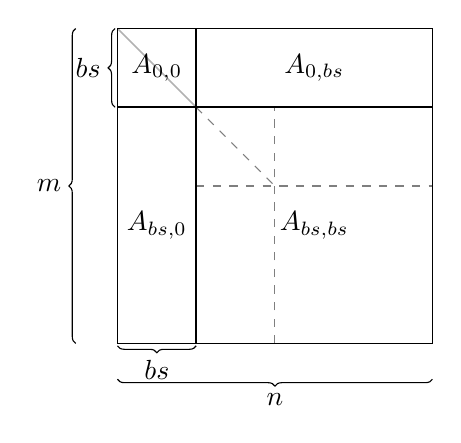
\begin{tikzpicture}
\draw[semithick] (0,0) -- (4,0) -- (4,4) -- (0,4) -- (0,0);

\draw[semithick] (1,0) -- (1,4);
\draw[semithick] (0,3) -- (4,3);
\draw[semithick,opacity=0.3] (0,4) -- (1,3);

\draw[dashed,opacity=0.5] (2,0) -- (2,3);
\draw[dashed,opacity=0.5] (1,2) -- (4,2);
\draw[dashed,opacity=0.5] (1,3) -- (2,2);


\draw (0.5,3.5) node {$A_{0,0}$};
\draw (0.5,1.5) node {$A_{bs,0}$};
\draw (2.5,3.5) node {$A_{0,bs}$};
\draw (2.5,1.5) node {$A_{bs,bs}$};
\draw[decorate, decoration={brace,mirror}, yshift=-.2ex]  (0,0) -- node[below=0.4ex] {$bs$}  (1,0);
\draw[decorate, decoration={brace}, xshift=-.2ex]  (0,3) -- node[left=0.4ex] {$bs$}  (0,4);
\draw[decorate, decoration={brace,mirror}, yshift=-3ex]  (0,0) -- node[below=0.4ex] {$n$}  (4,0);
\draw[decorate, decoration={brace}, xshift=-3.5ex]  (0,0) -- node[left=0.4ex] {$m$}  (0,4);

\end{tikzpicture}